\documentclass{labs}

\usepackage{cmap} % чтобы работал поиск по PDF

\usepackage{ulem}\normalem

\pdfcompresslevel=9 % сжимать PDF
\usepackage{pdflscape} % для возможности альбомного размещения некоторых страниц
\usepackage[pdftex]{hyperref}
% настройка ссылок в оглавлении для pdf формата
\hypersetup{unicode=true,
  pdftitle={Вычислителньые системы. Лаба1},
    pdfauthor={Погода Михайло},
    pdfcreator={pdflatex},
    pdfsubject={},
    pdfborder    = {0 0 0},
    bookmarksopen,
    bookmarksnumbered,
    bookmarksopenlevel = 2,
    pdfkeywords={},
    colorlinks=true, % установка цвета ссылок в оглавлении
    citecolor=black, 
    filecolor=black,
    linkcolor=black,
    urlcolor=blue
}

\usepackage{amsmath}
\usepackage{amssymb}
\usepackage{moreverb}

\author{Михаил Погода}
\title{Вычислительные системы. Лаба \textnumero~1}
\date{\today}

\begin{document}

\maketitlepage{1}{КОМБІНАЦІЙНІ СХЕМИ. МІНІМІЗАЦІЯ ПЕРЕМИКАЛЬНИХ ФУНКЦІЙ}{Погода~М.\,В.}{КМ-92}

\intro

  У цій лабораторній роботі необхідно виконати синтез комбінаційної схеми на
  базисі заданої системи перемикальних функцій, а потім визначити її основні
  параметри, такі як складність і швидкодія.
  Під час синтезу схеми потрібно виконати порівняльний
  аналіз різних варіантів побудови комбінаційної схеми та обрати оптимальний.
\newpage

\chapter{Постановка задачі}
  \begin{enumerator}
    \item Мінімізувати кожну з перемикальних функцій, заданих в таблиці на
      рис.~\ref{task-table}, деяким методом мінімізації (Квайна, невизначених
      коефіцієнтів, діаграм Вейча).
    \item Представити кожну з функцій у вісьмох нормальних операторних формах.
    \item Побудувати всі можливі види комбінаційних схем згідно з заданим
      операторним базисом.
    \item Визначити параметри складності, середній та максимальний час затримки
      схеми.
    \item Визначити найменш складну та найбільш швидкодіючу комбінаційну схеми
      та реалізувати їх у програмному комплексі \texttt{AFDK2.0}.
  \end{enumerator}

  \begin{supertable}{|c c c|c c c|}{6}{Таблиця істинності функцій}{task-table}
    \hline
    $x$&$y$&$z$& $f_1$ & $f_2$ & $f_3$ \\
    \hline
    $0$&$0$&$0$&$0$&$1$&$1$\\
    $0$&$0$&$1$&$1$&$0$&$0$\\
    $0$&$1$&$0$&$1$&$0$&$1$\\
    $0$&$1$&$1$&$0$&$1$&$1$\\
    $1$&$0$&$0$&$1$&$0$&$0$\\
    $1$&$0$&$1$&$0$&$0$&$1$\\
    $1$&$1$&$0$&$1$&$0$&$1$\\
    $1$&$1$&$1$&$0$&$1$&$0$\\
  \end{supertable}

  Базис, в якому треба будувати комбінаційну схему: 3АБО, 2І-НЕ.

  Часи затримки $t_{01}$ і $t_{10}$ покласти наступні:
  \begin{itemizer}
    \item для І-НЕ: 8 і 12 відповідно;
    \item для АБО: 10 і 14 відповідно.
  \end{itemizer}

\newpage
\chapter{Теоретичні відомості}
  Синтез комбінаційної схеми розбивається на три етапи:
  \begin{enumerator}
    \item Мінімізація функцій.
    \item Представлення функцій в операторній формі.
    \item Складання схеми.
  \end{enumerator}

  \section{Мінімізація перемикальних функцій}
    Під час виконання даної роботи ми розглянули три методи мінімізації
    функцій.
    Усі вони так чи інакше базуються на двох законах булевої алгебри --- законі
    повного склеювання:
    \begin{equation}
      xy\lor\bar{x}y = y
      \label{th1}
    \end{equation}
    та законі поглинання:
    \begin{equation}
      x \lor xy = x
      \label{th2}
    \end{equation}

    Одним з методів мінімізації є \textit{метод Квайна}.
    Його ідея полягає в тому, щоб шляхом застосування законів (\ref{th1}) та
    (\ref{th2}) звести початкову ДДНФ функції до СДНФ.
    У процесі мінімізації за методом Квайна потрібно виконати наступні кроки:
    \begin{enumerator} 
      \item Записати ДДНФ заданої функції.
      \item Застосувати закони склеювання та поглинання послідовно до
        конституент одиниці, а потім ітеративно до отриманих імплікант.
      \item Побудувати таблицю покриття (імплікантну матрицю) та знайти ТДНФ..
      \item Вибрати з числа ТДНФ ДНФ з мінімальною ціною.
    \end{enumerator}

    Ще одним методом мінімізації функцій є \textit{метод невизначених
    коефіцієнтів}.
    Останнім з методів мінімізації перемикальних функцій є \textit{метод діаграм
    Вейча}.
    Етапи мінімізації при використанні діаграм Вейча:
    \begin{enumerator}
      \item Заповнення діаграми Вейча значеннями функції, яких вона набуває на
        відповідних наборах.
      \item Об’єднання всіх одиниць у прямокутники з максимально можливою
        кількістю клітинок, при чому в кожному прямокутнику має бути $2^k$
        клітинок.
      \item Визначення МДНФ з мінімальної множини прямокутників, що покривають
        усі одиниці.
    \end{enumerator}

  \section{Представлення функцій в операторній формі}
    Отримання операторного представлення функції зводиться до її представлення в
    одній із нормальних форм.
    У базисі логічних елементів І, АБО, І-НЕ, АБО-НЕ таких нормальних форм
    вісім.
    Усі вони отримуються з ДНФ заданої функції шляхом послідовного використання
    правил де Моргана:
    \begin{equation}
      \overline{x \lor y} = \bar{x}\bar{y}, \quad \overline{xy} = \bar{x}\lor\bar{y}
    \end{equation}

  \section{Складання схеми за критерієм оптимальності} 
  В даній лабораторній роботі ми порівнюємо схеми за оптимальністю та
  швидкодією.
  Існують різні способи оцінки складності схеми:
  \begin{enumerator}
    \item Оцінка за Квайном, $K$ --- сумарне число входів усіх логічних
      елементів комбінаційної схеми.
    \item Складність як загальне число логічних елементів.
    \item Складність як число $N$ умовних логічних елементів, що розраховується
      за формулою:
    \begin{equation}
      N = \sum_{i = 1}^r\frac{m_i n_i}{g}
    \end{equation}
    де $r$ --- число типів елементів, $m_i$, $n_i$ --- число елементів $і$-го
    типу та входів цього елемента, $g$ --- число входів умовного елемента.
  \end{enumerator}

  Швидкодію комбінаційної схеми визначають часові параметри логічних елементів, що характеризують
  час переходу схеми з одного стану в інший.
  На практиці використовують максимальне значення часу затримки
  $t = \max(t_{01}, t_{10})$, або усереднений час затримки
  $t = \frac{t_{01} + t_{10}}{2}$.
  Середній час затримки всієї комбінаційної схеми дорівнює сумі часових затримок окремих
  елементів на тому шляху, який вимагає максимального часу поширення сигналу.

\newpage
\chapter{Практичні результати}
  \section{Функція $f_1$}

    \begin{supertable}{|c c c|c|}{4}{Таблиця істинності функції $f_1$}{table-f1}
      \hline
      $x$&$y$&$z$&$f_1$\\
      \hline
      $0$&$0$&$0$&$0$\\
      $0$&$0$&$1$&$1$\\
      $0$&$1$&$0$&$1$\\
      $0$&$1$&$1$&$0$\\
      $1$&$0$&$0$&$1$\\
      $1$&$0$&$1$&$0$\\
      $1$&$1$&$0$&$1$\\
      $1$&$1$&$1$&$0$\\
    \end{supertable}

    $$ \text{ДДНФ}: f_1 = \bar{x}\bar{y}z \lor \bar{x}y\bar{z} \lor
        x\bar{y}\bar{z} \lor xy\bar{z}$$

    Після склеювання другої та четвертої імплікант, будемо мати:
  $$f_1 = \bar{x}\bar{y}z \lor x\bar{y}\bar{z} \lor y\bar{z}$$

    Представимо функцію у вісьмох нормальних формах:

    $$
    \begin{array}{rl}
      f_1 &= \bar{x}\bar{y}z \lor x\bar{y}\bar{z} \lor y\bar{z}\\
          &= \overline{\strut\overline{\strut\bar{x}\bar{y}z} \cdot
             \overline{\strut x\bar{y}\bar{z}} \cdot \overline{\strut y\bar{z}}}\\
          &= \overline{\strut(x \lor y \lor \bar{z})
             (\bar{x} \lor y \lor z)
             (\bar{y} \lor z)}\\
          &= \overline{\strut(x \lor y \lor \bar{z})} \lor
             \overline{\strut(\bar{x} \lor y \lor z)} \lor
             \overline{\strut(\bar{y} \lor z)}\\
          &= \overline{\strut\bar{x}\bar{y}\bar{z} \lor yz \lor xz}\\
          &= \overline{\strut\bar{x}\bar{y}\bar{z}} \cdot
             \overline{\strut yz} \cdot \overline{\strut xz}\\
          &= (x \lor y \lor z)(\bar{y} \lor \bar{z})(\bar{x} \lor \bar{z})\\
          &= \overline{\strut\overline{\strut(x \lor y \lor z)} \lor
             \overline{\strut(\bar{y} \lor \bar{z})} \lor
             \overline{\strut(\bar{x} \lor \bar{z})}}
    \end{array}
    $$

  \section{Функція $f_2$}

    \begin{supertable}{|c c c|c|}{4}{Таблиця істинності функції $f_2$}{table-f2}
      \hline
      $x$&$y$&$z$&$f_2$\\
      \hline
      $0$&$0$&$0$&$1$\\
      $0$&$0$&$1$&$0$\\
      $0$&$1$&$0$&$0$\\
      $0$&$1$&$1$&$1$\\
      $1$&$0$&$0$&$0$\\
      $1$&$0$&$1$&$0$\\
      $1$&$1$&$0$&$0$\\
      $1$&$1$&$1$&$1$\\
    \end{supertable}

    \begin{supertable}{|c c c | c c c c c c  c |c|}{10}{Таблиця невизначених коефіцієнтів для функції $F_2$}{table-coef-f2}
      \hline
      $x$&$y$&$z$&\multicolumn{7}{|c|}{Коефіцієнти}&$f_2$\\
      \hline
      $0$ & $0$ & $0$	&\xout{$k_x^0$} &\xout{$k_y^0$} &\xout{$k_z^0$} &\xout{$k_{xy}^{00}$} &\xout{$k_{xz}^{00}$} &\xout{$k_{yz}^{00}$} &$k_{xyz}^{000}$        &$1$\\
      $0$ & $0$ & $1$	&\xout{$k_x^0$} &\xout{$k_y^0$} &\xout{$k_z^1$} &\xout{$k_{xy}^{00}$} &\xout{$k_{xz}^{01}$} &\xout{$k_{yz}^{01}$} &\xout{$k_{xyz}^{001}$} &$0$\\
      $0$ & $1$ & $0$	&\xout{$k_x^0$}	&\xout{$k_y^1$} &\xout{$k_z^0$} &\xout{$k_{xy}^{01}$} &\xout{$k_{xz}^{00}$} &\xout{$k_{yz}^{10}$} &\xout{$k_{xyz}^{010}$} &$0$\\
      $0$ & $1$ & $1$	&\xout{$k_x^0$}	&\xout{$k_y^1$} &\xout{$k_z^1$} &\xout{$k_{xy}^{01}$} &\xout{$k_{xz}^{01}$} &$k_{yz}^{11}$        &$k_{xyz}^{011}$        &$1$\\
      $1$ & $0$ & $0$	&\xout{$k_x^1$}	&\xout{$k_y^0$} &\xout{$k_z^0$} &\xout{$k_{xy}^{10}$} &\xout{$k_{xz}^{10}$} &\xout{$k_{yz}^{00}$} &\xout{$k_{xyz}^{100}$} &$0$\\
      $1$ & $0$ & $1$	&\xout{$k_x^1$}	&\xout{$k_y^0$} &\xout{$k_z^1$} &\xout{$k_{xy}^{10}$} &\xout{$k_{xz}^{11}$} &\xout{$k_{yz}^{01}$} &\xout{$k_{xyz}^{101}$} &$0$\\
      $1$ & $1$ & $0$	&\xout{$k_x^1$}	&\xout{$k_y^1$} &\xout{$k_z^0$} &\xout{$k_{xy}^{11}$} &\xout{$k_{xz}^{10}$} &\xout{$k_{yz}^{10}$} &\xout{$k_{xyz}^{110}$} &$0$\\
      $1$ & $1$ & $1$	&\xout{$k_x^1$}	&\xout{$k_y^1$} &\xout{$k_z^1$} &\xout{$k_{xy}^{11}$} &\xout{$k_{xz}^{11}$} &$k_{yz}^{11}$        &$k_{xyz}^{111}$        &$1$\\			
    \end{supertable}

    Отримаємо коефіцієнти, що утворюють CДНФ:
    $$f_2 = \bar{x}\bar{y}\bar{z} \lor yz$$

    Представимо функцію у вісьмох нормальних формах:

    $$
    \begin{array}{rl}
      f2 &= \bar{x}\bar{y}\bar{z} \lor yz\\
         &= \overline{\strut\overline{\strut\bar{x}\bar{y}\bar{z}} \cdot \overline{\strut yz}}\\
         &= \overline{\strut(x \lor y \lor z) (\bar{y} \lor \bar{z})}\\
         &= \overline{\strut(x \lor y \lor z)} \lor \overline{\strut(\bar{y}\lor\bar{z})}\\
         &= \overline{\strut y\bar{z} \lor x\bar{z} \lor \bar{y}z \lor \bar{y}x}\\
         &= \overline{\strut y\bar{z}} \cdot \overline{\strut x\bar{z}} \cdot \overline{\strut \bar{y}z} \cdot \overline{\strut\bar{y}x}\\
         &= (\bar{y} \lor z)(\bar{x} \lor z)(y \lor \bar{z})(y \lor \bar{x})\\
         &= \overline{\strut\overline{\strut(\bar{y} \lor z)} \lor \overline{\strut(\bar{x} \lor z)} \lor \overline{\strut(y \lor \bar{z})} \lor \overline{\strut(y \lor \bar{x})}}\\
    \end{array}
    $$

  \section{Функція $f_3$}

    \begin{supertable}{|c c c|c|}{4}{Таблиця істинності функції $f_3$}{table-f3}
      \hline
      $x$&$y$&$z$&$f_3$\\
      \hline
      $0$&$0$&$0$&$1$\\
      $0$&$0$&$1$&$0$\\
      $0$&$1$&$0$&$1$\\
      $0$&$1$&$1$&$1$\\
      $1$&$0$&$0$&$0$\\
      $1$&$0$&$1$&$1$\\
      $1$&$1$&$0$&$1$\\
      $1$&$1$&$1$&$0$\\
    \end{supertable}


    $$\text{ДДНФ}: f_3 = \bar{x}\bar{y}\bar{z} \lor \bar{x}y\bar{z} \lor \bar{x}yz \lor x\bar{y}z \lor xy\bar{z}$$

    Мінімізуємо функцію з допомогою діаграм Вейча:

    \begin{figure}[ht]
      \centering
      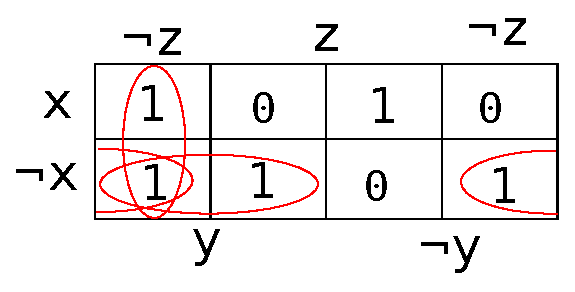
\includegraphics{veich.eps}
      \caption{Діаграма Вейча для $f_3$}
      \label{veich-f3}
    \end{figure}

    $$\text{МДНФ}: f_3 = \bar{x}y \lor y\bar{z} \lor \bar{x}\bar{z} \lor x\bar{y}z$$

    Представимо функцію у вісьмох нормальних формах:

    $$
    \begin{array}{rl}
      f_3 &= \bar{x}y \lor y\bar{z} \lor \bar{x}\bar{z} \lor x\bar{y}\\
          &= \overline{\strut\overline{\strut\bar{x}y} \cdot \overline{\strut\bar{x}\bar{z}} \cdot \overline{\strut y\bar{z}} \cdot \overline{\strut x\bar{y}z}}\\
          &= \overline{\strut(x\lor\bar{y})(x\lor z)(\bar{y}\lor z)(\bar{x}\lor y\lor\bar{z})}\\
          &= \overline{\strut(x\lor\bar{y})} \lor \overline{\strut(x\lor z)} \lor \overline{\strut(\bar{y}\lor z)} \lor \overline{\strut(\bar{x}\lor y\lor\bar{z})}\\
          &= \overline{\strut \bar{x}\bar{y}z \lor x\bar{y}\bar{z} \lor xyz}\\
          &= \overline{\strut\bar{x}\bar{y}z} \cdot \overline{\strut x\bar{y}\bar{z}} \cdot \overline{\strut xyz}\\
          &= (x \lor y \lor \bar{z})(\bar{x} \lor y \lor z)(\bar{x} \lor \bar{y} \lor \bar{z})\\
          &= \overline{\strut\overline{\strut(x \lor y \lor \bar{z})} \lor \overline{\strut(\bar{x} \lor y \lor z)} \lor \overline{\strut(\bar{x} \lor \bar{y} \lor \bar{z})}}\\
    \end{array}
    $$

  \newpage
  \section{Складання схеми згiдно з критерiєм оптимальності}

  \begin{figure}[ht]
    \centering
    \includegraphics[scale=0.65]{lab1.png}
    \caption{Комбінаційна схема}
    \label{schema}
  \end{figure}	

  \begin{supertable}{|c|c|c|c|c|}{5}{Таблиця параметрів КС}{schema-params}
    \hline
    $K$ & $G$ & $N$ & Максимальний час & Середній час\\
    \hline
    $34$ & $14$ & $16.5$ & $40$ & $34$\\
  \end{supertable}

\newpage
\chapter{Висновки}

  У цій лабораторній роботі був проведений синтез комбінаційної схеми на базисі
  заданої системи перемикальних функцій.
  Синтез складався з декількох основних етапів:
  \begin{enumerator}
    \item Мінімізації функції (одним з запропонованих методів).
    \item Визначення нормальних операторних форм функції (необхідний для
      представлення функції в заданому базисі).
    \item Побудова комбінаційної схеми в комплексі \texttt{AFDK2.0}.
    \item Визначення параметрів комбінаційної схеми.
    \item Аналіз і визначення оптимальної комбінаційної схеми.	
  \end{enumerator}

  Оптимальну схему слід вибирати в залежності від того, який з параметрів має
  більше значення: швидкодія чи дешевизна.
  У моєму випадку, оптимальна схема має меншу кількість елементів й більшу
  швидкість, тобто немає альтернатив.

\end{document}
